\documentclass[12pt,letterpaper]{article}
\usepackage{graphicx,textcomp}
\usepackage{natbib}
\usepackage{setspace}
\usepackage{fullpage}
\usepackage{color}
\usepackage[reqno]{amsmath}
\usepackage{amsthm}
\usepackage{fancyvrb}
\usepackage{amssymb,enumerate}
\usepackage[all]{xy}
\usepackage{endnotes}
\usepackage{lscape}
\newtheorem{com}{Comment}
\usepackage{float}
\usepackage{hyperref}
\newtheorem{lem} {Lemma}
\newtheorem{prop}{Proposition}
\newtheorem{thm}{Theorem}
\newtheorem{defn}{Definition}
\newtheorem{cor}{Corollary}
\newtheorem{obs}{Observation}
\usepackage[compact]{titlesec}
\usepackage{dcolumn}
\usepackage{tikz}
\usetikzlibrary{arrows}
\usepackage{multirow}
\usepackage{xcolor}
\newcolumntype{.}{D{.}{.}{-1}}
\newcolumntype{d}[1]{D{.}{.}{#1}}
\definecolor{light-gray}{gray}{0.65}
\usepackage{url}
\usepackage{listings}
\usepackage{color}

\definecolor{codegreen}{rgb}{0,0.6,0}
\definecolor{codegray}{rgb}{0.5,0.5,0.5}
\definecolor{codepurple}{rgb}{0.58,0,0.82}
\definecolor{backcolour}{rgb}{0.95,0.95,0.92}

\lstdefinestyle{mystyle}{
	backgroundcolor=\color{backcolour},   
	commentstyle=\color{codegreen},
	keywordstyle=\color{magenta},
	numberstyle=\tiny\color{codegray},
	stringstyle=\color{codepurple},
	basicstyle=\footnotesize,
	breakatwhitespace=false,         
	breaklines=true,                 
	captionpos=b,                    
	keepspaces=true,                 
	numbers=left,                    
	numbersep=5pt,                  
	showspaces=false,                
	showstringspaces=false,
	showtabs=false,                  
	tabsize=2
}
\lstset{style=mystyle}
\newcommand{\Sref}[1]{Section~\ref{#1}}
\newtheorem{hyp}{Hypothesis}

\title{Problem Set 3}
\date{Due: November 11, 2024}
\author{Applied Stats/Quant Methods 1}


\begin{document}
	\maketitle
	\section*{Instructions}
	\begin{itemize}
		\item Please show your work! You may lose points by simply writing in the answer. If the problem requires you to execute commands in \texttt{R}, please include the code you used to get your answers. Please also include the \texttt{.R} file that contains your code. If you are not sure if work needs to be shown for a particular problem, please ask.
	\item Your homework should be submitted electronically on GitHub.
	\item This problem set is due before 23:59 on Sunday November 11, 2024. No late assignments will be accepted.

	\end{itemize}

		\vspace{.25cm}
	
\noindent In this problem set, you will run several regressions and create an add variable plot (see the lecture slides) in \texttt{R} using the \texttt{incumbents\_subset.csv} dataset. Include all of your code.

	\vspace{.5cm}
\section*{Question 1}
\vspace{.25cm}
\noindent We are interested in knowing how the difference in campaign spending between incumbent and challenger affects the incumbent's vote share. 
	\begin{enumerate}
		\item Run a regression where the outcome variable is \texttt{voteshare} and the explanatory variable is \texttt{difflog}.	
		
		\lstinputlisting[language=R, firstline=36, lastline=41]{PS3.R} 
		
		Then we can get
		
		Call:\\
		lm(formula = voteshare \~{} difflog, data = inc.sub)\\
		
		Residuals:\\
			\begin{verbatim}
		     Min       1Q   Median       3Q      Max 
		-0.26832 -0.05345 -0.00377  0.04780  0.32749 
		\end{verbatim}
		
		Coefficients:\\
		\begin{verbatim}
			            Estimate Std. Error t value Pr(>|t|)    
			(Intercept) 0.579031   0.002251  257.19   <2e-16 ***
			difflog     0.041666   0.000968   43.04   <2e-16 ***
		\end{verbatim}
		
		---
		Signif. codes:  0 ‘***’ 0.001 ‘**’ 0.01 ‘*’ 0.05 ‘.’ 0.1 ‘ ’ 1
		
		Residual standard error: 0.07867 on 3191 degrees of freedom
		Multiple R-squared:  0.3673,	Adjusted R-squared:  0.3671 
		F-statistic:  1853 on 1 and 3191 DF,  p-value: $<$ 2.2e-16
		
		We can see the coefficient for difflog is positive and statistically significant, so higher campaign spending relative to the challenger (a higher difflog value) is associated with an increased vote share for the incumbent.
		
\vspace{5cm}
		\item Make a scatterplot of the two variables and add the regression line. 	
		
			\lstinputlisting[language=R, firstline=48, lastline=57]{PS3.R} 
			
		\begin{figure}[H]\centering
			
			\label{fig:plot_1}
			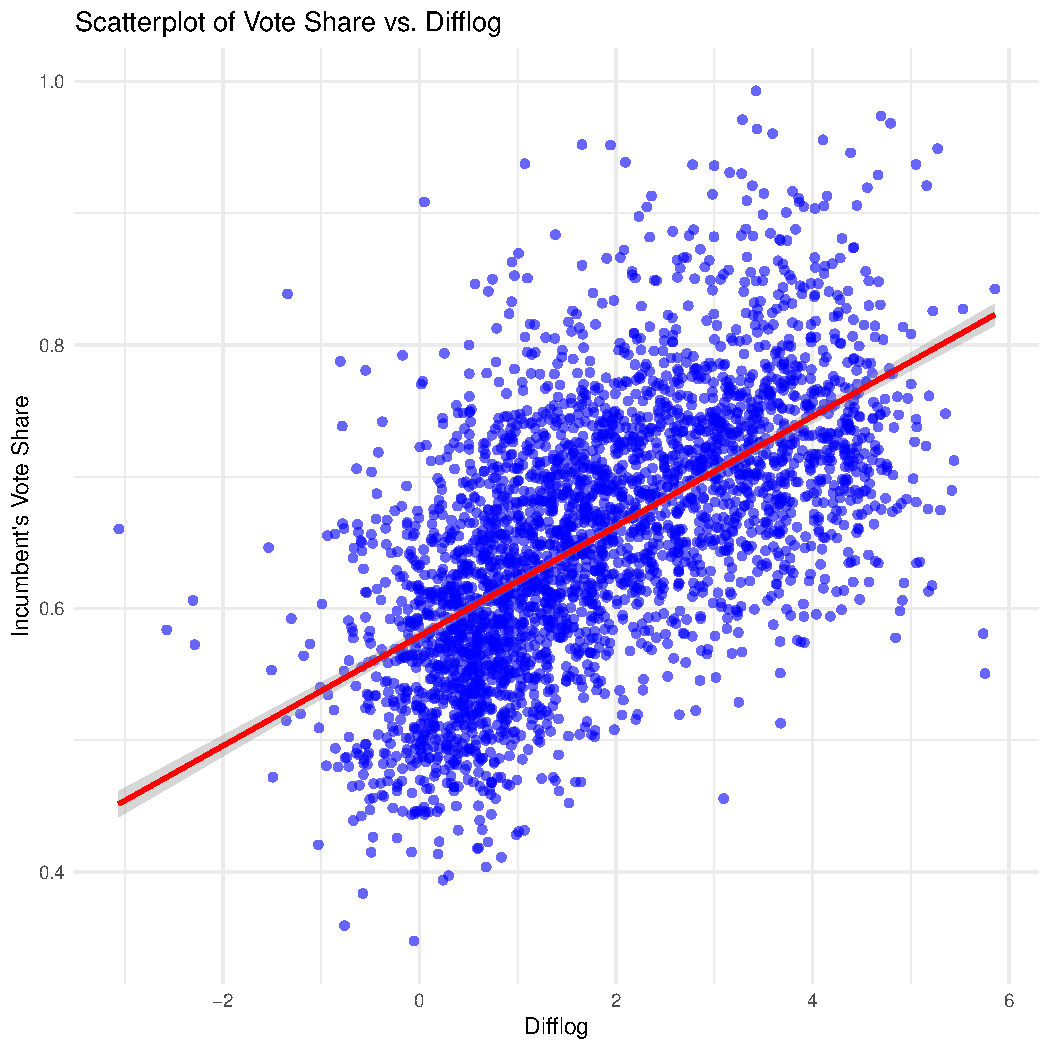
\includegraphics[width=.55\textwidth]{Scatterplot with regression line.pdf}
		\end{figure}
		\vspace{3cm}
		\item Save the residuals of the model in a separate object.						\lstinputlisting[language=R, firstline=59, lastline=63]{PS3.R} 
			\begin{verbatim}
     1             2             3            
    -0.0004227622 -0.0316840149 -0.0045514943  
		\end{verbatim}
		\begin{verbatim}
     4             5             6 
	  0.0386688767  0.0355287965  0.0322832521 
		\end{verbatim}
		\vspace{7cm}

		
		\item Write the prediction equation.
		
		voteshare=0.579031+0.041666×difflog
		
	\end{enumerate}
	
\newpage

\section*{Question 2}
\noindent We are interested in knowing how the difference between incumbent and challenger's spending and the vote share of the presidential candidate of the incumbent's party are related.	\vspace{.25cm}
	\begin{enumerate}
		\item Run a regression where the outcome variable is \texttt{presvote} and the explanatory variable is \texttt{difflog}.
		
			\lstinputlisting[language=R, firstline=66, lastline=71]{PS3.R} 
			
			Then we can get\\
			
		Call:\\
		lm(formula = presvote \~{} difflog, data = inc.sub)\\
		
		
		Residuals:\\
			\begin{verbatim}
		 Min       1Q   Median       3Q      Max 
		-0.32196 -0.07407 -0.00102  0.07151  0.42743 
		\end{verbatim}
		Coefficients:\\
			\begin{verbatim}
	            	Estimate Std. Error t value Pr(>|t|)    
		(Intercept) 0.507583   0.003161  160.60   <2e-16 ***
		difflog     0.023837   0.001359   17.54   <2e-16 ***
		\end{verbatim}
		---\\
		Signif. codes:  0 ‘***’ 0.001 ‘**’ 0.01 ‘*’ 0.05 ‘.’ 0.1 ‘ ’ 1\\
		
		Residual standard error: 0.1104 on 3191 degrees of freedom\\
		Multiple R-squared:  0.08795,	Adjusted R-squared:  0.08767 \\
		F-statistic: 307.7 on 1 and 3191 DF,  p-value: $<$ 2.2e-16\\
		
		We can see the coefficient for difflog is positive and statistically significant, so higher campaign spending relative to the challenger (a higher difflog value) is associated with presvote.
			\vspace{5cm}
		\item Make a scatterplot of the two variables and add the regression line. 
			\lstinputlisting[language=R, firstline=73, lastline=82]{PS3.R} 
			\begin{figure}[H]\centering
			
			\label{fig:plot_2}
			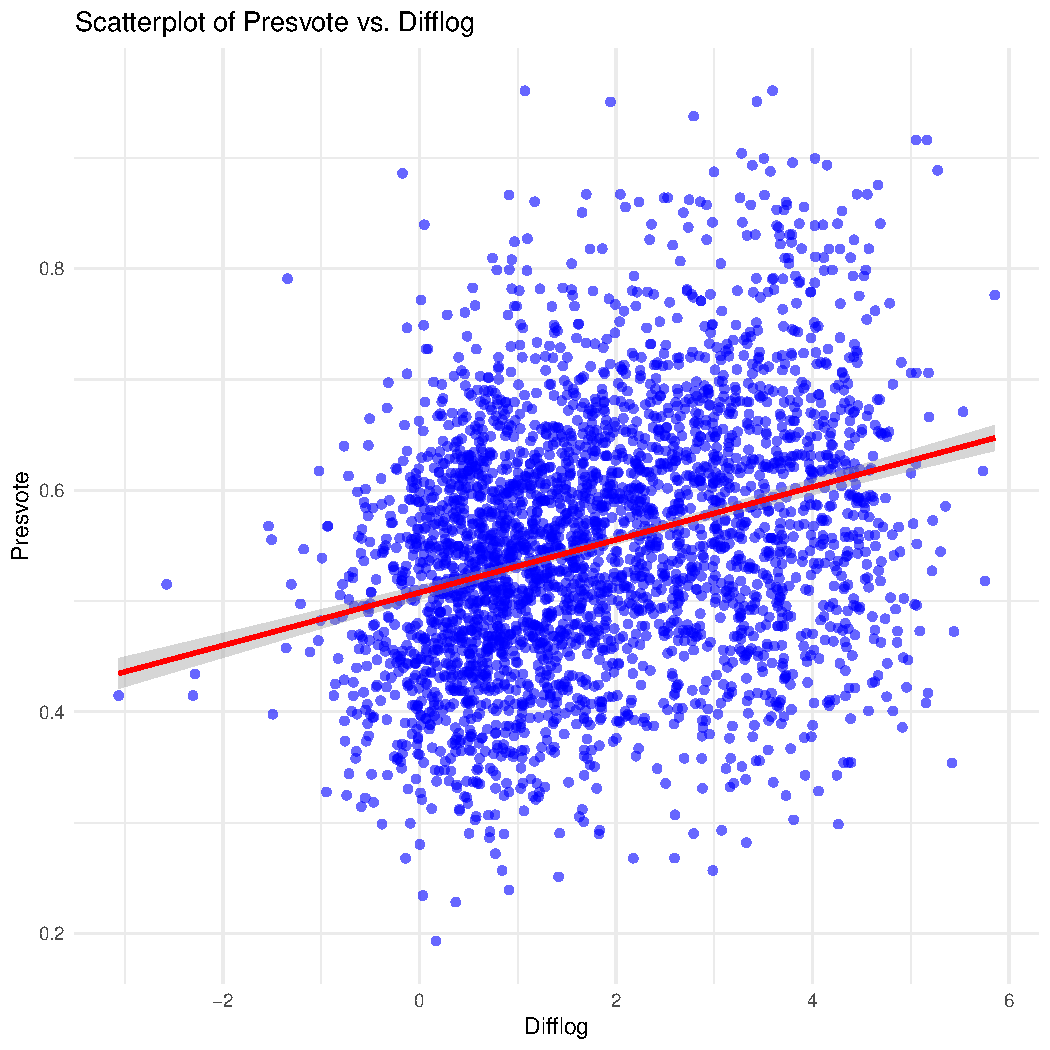
\includegraphics[width=.55\textwidth]{Scatterplot with regression line2.pdf}
		\end{figure}
			\vspace{5cm}
		\item Save the residuals of the model in a separate object.	
			\lstinputlisting[language=R, firstline=84, lastline=88]{PS3.R} 
				\begin{verbatim}
			  1            2            3       
			0.005605594  0.037578519 -0.053134788
			\end{verbatim}
			\begin{verbatim}
				4             5             6 
			-0.052993694 -0.045842994  0.074339701
			\end{verbatim}
		\vspace{5cm}
		\item Write the prediction equation.
		
		presvote=0.507583+0.023837×difflog
	\end{enumerate}
	
	\newpage	
\section*{Question 3}

\noindent We are interested in knowing how the vote share of the presidential candidate of the incumbent's party is associated with the incumbent's electoral success.
	\vspace{.25cm}
	\begin{enumerate}
		\item Run a regression where the outcome variable is \texttt{voteshare} and the explanatory variable is \texttt{presvote}.
			\lstinputlisting[language=R, firstline=90, lastline=95]{PS3.R} 
			
				Then we can get\\
			
			Call:\\
			lm(formula = voteshare \~{} presvote, data = inc.sub)\\
			
				Residuals:\\
			\begin{verbatim}
				  Min       1Q   Median       3Q      Max 
				-0.27330 -0.05888  0.00394  0.06148  0.41365
			\end{verbatim}
			Coefficients:\\
			\begin{verbatim}
		            	Estimate Std. Error t value Pr(>|t|)    
			(Intercept) 0.441330   0.007599   58.08   <2e-16 ***
			presvote    0.388018   0.013493   28.76   <2e-16 ***
			\end{verbatim}
			---\\
			Signif. codes:  0 ‘***’ 0.001 ‘**’ 0.01 ‘*’ 0.05 ‘.’ 0.1 ‘ ’ 1\\
			
			Residual standard error: 0.08815 on 3191 degrees of freedom\\
			Multiple R-squared:  0.2058,	Adjusted R-squared:  0.2056 \\
			F-statistic:   827 on 1 and 3191 DF,  p-value: $<$ 2.2e-16\\
			
			We can see the coefficient for presvote is positive and statistically significant, so presvote is associated with voteshare.
				
			\vspace{5cm}
			
		\item Make a scatterplot of the two variables and add the regression line. 
			\lstinputlisting[language=R, firstline=97, lastline=106]{PS3.R} 
			\begin{figure}[H]\centering
			
			\label{fig:plot_3}
			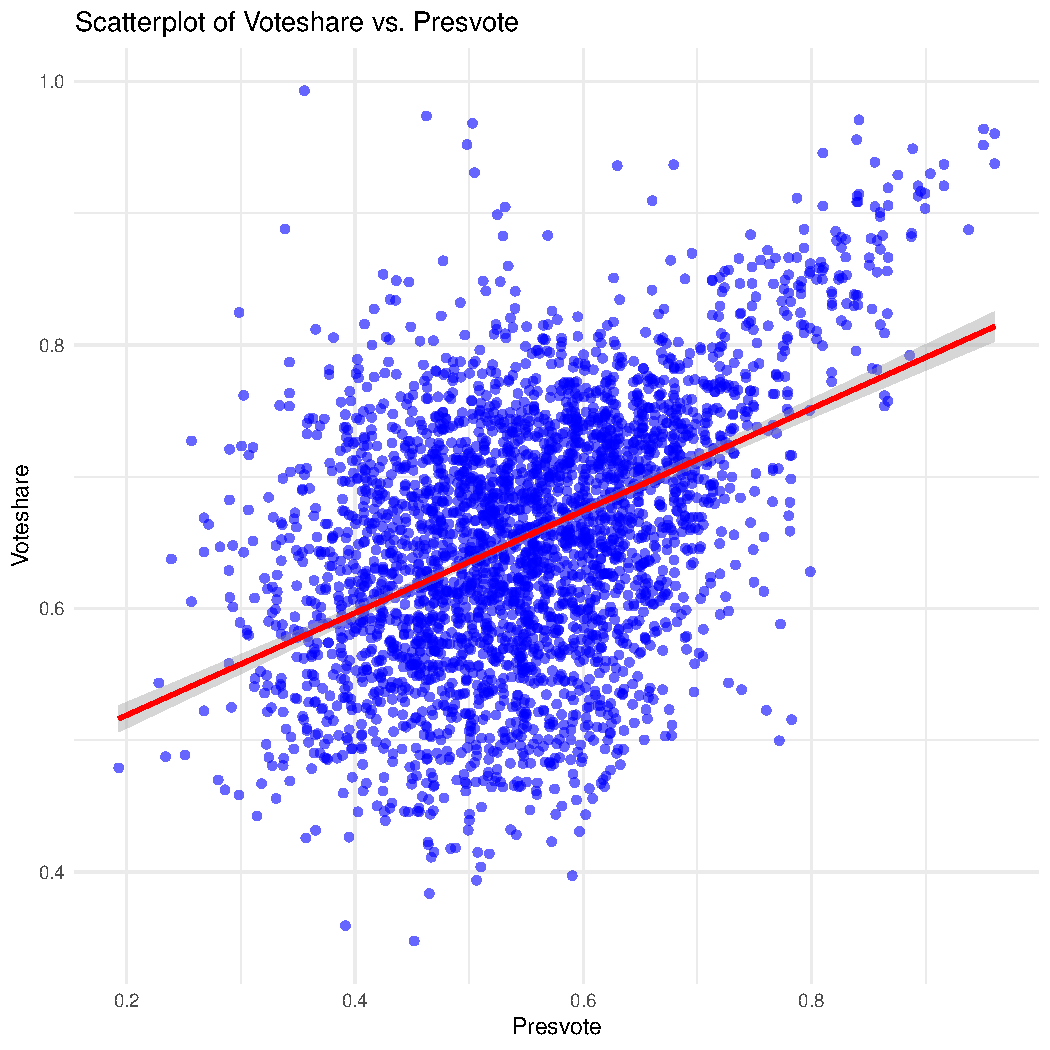
\includegraphics[width=.55\textwidth]{Scatterplot with regression line3.pdf}
		\end{figure}
			\vspace{6cm}
		\item Write the prediction equation.
		
		voteshare=0.441330+0.388018×presvote
	\end{enumerate}
	

\newpage	
\section*{Question 4}
\noindent The residuals from part (a) tell us how much of the variation in \texttt{voteshare} is $not$ explained by the difference in spending between incumbent and challenger. The residuals in part (b) tell us how much of the variation in \texttt{presvote} is $not$ explained by the difference in spending between incumbent and challenger in the district.
	\begin{enumerate}
		\item Run a regression where the outcome variable is the residuals from Question 1 and the explanatory variable is the residuals from Question 2.	
		\lstinputlisting[language=R, firstline=108, lastline=113]{PS3.R} 
		
			Then we can get\\
		
		Call:\\
		lm(formula = residuals\_model \~{} residuals\_model2, data = inc.sub)\\
		
			Residuals:\\
		\begin{verbatim}
		     Min       1Q   Median       3Q      Max 
		-0.25928 -0.04737 -0.00121  0.04618  0.33126 
		\end{verbatim}
		Coefficients:\\
		\begin{verbatim}
		                 Estimate Std. Error t value Pr(>|t|)    
		(Intercept)      -1.942e-18  1.299e-03    0.00        1    
		residuals_model2  2.569e-01  1.176e-02   21.84   <2e-16 ***
		\end{verbatim}
		---\\
		Signif. codes:  0 ‘***’ 0.001 ‘**’ 0.01 ‘*’ 0.05 ‘.’ 0.1 ‘ ’ 1\\
		
		Residual standard error: 0.07338 on 3191 degrees of freedom\\
		Multiple R-squared:   0.13,	Adjusted R-squared:  0.1298 \\
		F-statistic:   477 on 1 and 3191 DF,  p-value: $<$ 2.2e-16
		\vspace{6cm}
		\item Make a scatterplot of the two residuals and add the regression line. 
			\lstinputlisting[language=R, firstline=115, lastline=124]{PS3.R} 
			\begin{figure}[H]\centering
			
			\label{fig:plot_4}
			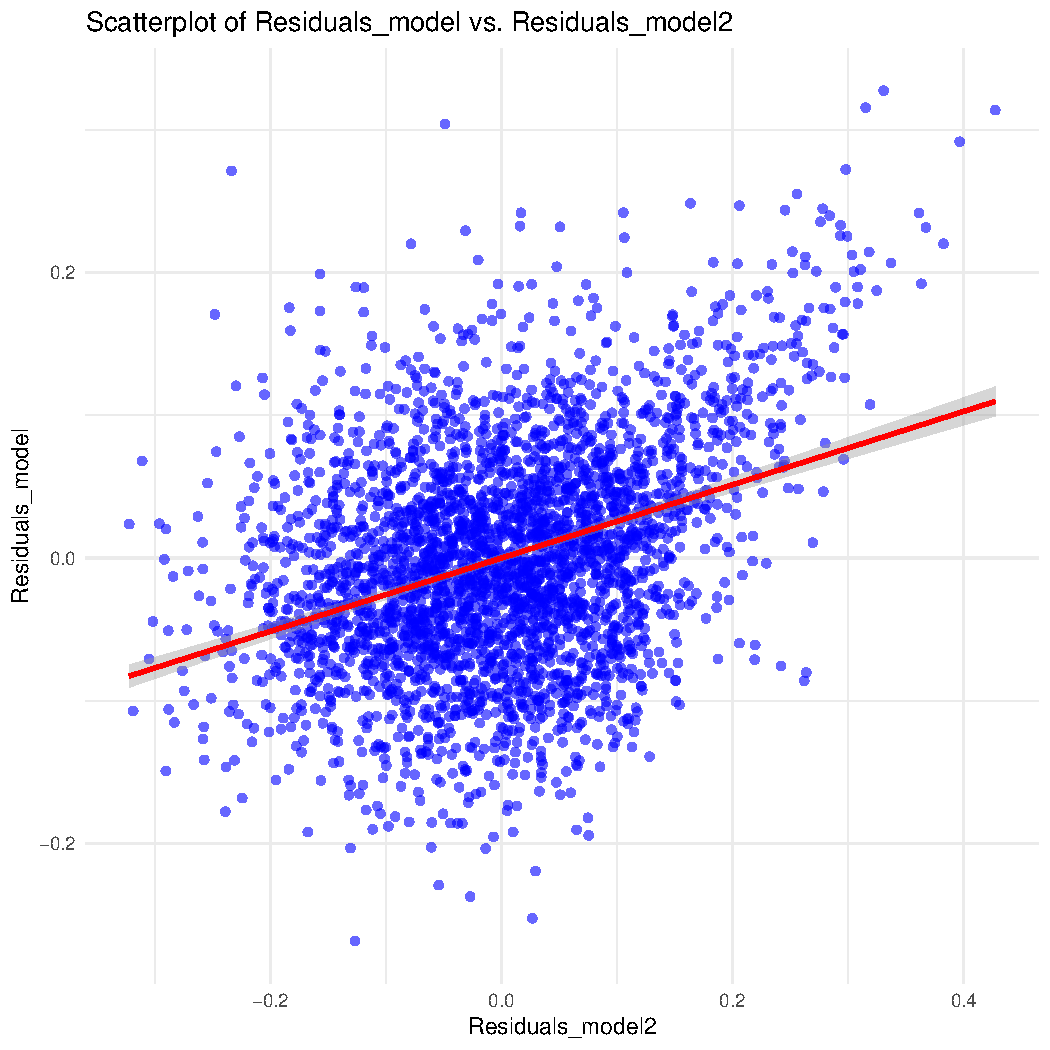
\includegraphics[width=.55\textwidth]{Scatterplot with regression line4.pdf}
				\end{figure}\vspace{6cm}
		\item Write the prediction equation.
		
		the residuals from Question 1=-1.942e-18+2.569e-01×the residuals from Question 2
	\end{enumerate}
	
	\newpage	

\section*{Question 5}
\noindent What if the incumbent's vote share is affected by both the president's popularity and the difference in spending between incumbent and challenger? 
	\begin{enumerate}
		\item Run a regression where the outcome variable is the incumbent's \texttt{voteshare} and the explanatory variables are \texttt{difflog} and \texttt{presvote}.	
			\lstinputlisting[language=R, firstline=126, lastline=131]{PS3.R} 
			
			Then we can get\\
			
			Call:\\
			lm(formula = voteshare \~{} difflog + presvote, data = inc.sub)\\
			
				Residuals:\\
			\begin{verbatim}
				  Min       1Q   Median       3Q      Max 
				-0.25928 -0.04737 -0.00121  0.04618  0.33126 
			\end{verbatim}
			Coefficients:\\
			\begin{verbatim}
             Estimate Std. Error t value Pr(>|t|)    
(Intercept) 0.4486442  0.0063297   70.88   <2e-16 ***
difflog     0.0355431  0.0009455   37.59   <2e-16 ***
presvote    0.2568770  0.0117637   21.84   <2e-16 ***
			\end{verbatim}
			---\\
			Signif. codes:  0 ‘***’ 0.001 ‘**’ 0.01 ‘*’ 0.05 ‘.’ 0.1 ‘ ’ 1\\
			
			Residual standard error: 0.07339 on 3190 degrees of freedom\\
			Multiple R-squared:  0.4496,	Adjusted R-squared:  0.4493 \\
			F-statistic:  1303 on 2 and 3190 DF,  p-value: $<$ 2.2e-16
		\vspace{5cm}
		\item Write the prediction equation.	
		
			voteshare=0.4486442+0.0355431×difflog+0.2568770×presvote
		\vspace{5cm}
		\item What is it in this output that is identical to the output in Question 4? Why do you think this is the case?
		
		The coefficient for presvote in the multiple regression of voteshare \~{} difflog + presvote should be identical to the coefficient from the residuals regression in Question 4.\\
		
		
		This process is known as partial regression or adjustment for other predictors in multiple regression, which explains why the coefficient of presvote in this multiple regression is identical to the coefficient in the residual regression from Question 4.
		
		
	\end{enumerate}




\end{document}
